%!TEX root = ../Thesis.tex

\chapter{Creating the Android app}
\label{android}
	So far we have only described our detection algorithm, but not how we gather the data and interact with the user. Our goal was to create a simple user experience showcasing the algorithm rather than building a full featured app. Still we wanted to hide the technical details as far as useful to stay reasonably close to a usable end product.

	The app was deployed and developed for a \textit{Nexus 4} (also known as \textit{LG-E960}) running \textit{Android Lollipop 5.0.1} build LRX22C.

	\section{Tethering in the framework}
	\label{android-framework}
	\subsection{Adding the source dependencies}
	\label{android-framework-dependencies}
	OpenCV for Android is available since September 2011 so we will not describe in detail how we set it up. In short the process is as following. The Android bindings for OpenCV can be downloaded from the official site and be compiled into a library which can then be included into one's project's \textit{lib}-folder. Alternatively the framework can be set as a dependency in Eclipse Android Development Tool and let it handle the compilation and dependency resolution, which is how we included the library.

	One could build all the OpenCV native code for the framework oneself. This implies building it for every possible target architecture (ARMv6, ARMv7, x86...) and shipping it with the app. This creates large binaries, at the benefit of having a standalone application. The recommended way on the other hand is to depend on the \textit{OpenCV Manager} app and ask the user on first start to install it, if necessary. This manager will then download the correct OpenCV native binaries in the required version and share it between all applications needing it. We chose to do the latter, at least for our prototype.

	\subsection{Gathering data}
	\label{android-framework-gathering}
	On Android apps are structured into \textit{Activities}. Those roughly correspond to the screens visible to a user: If an app that has an overview screen, an editor screen and a preview screen, it will likely have three activities.

	Each activity is built out of \textit{Views} describing and implementing the user interface. The OpenCV framework provides a special \texttt{JavaCameraView}. This view offers a callback to \texttt{CvCameraListener2} interfaces for the delivery of camera frames and displays them on the screen. However it does not expose access to the camera and locks the device for itself. To have more control over the camera we subclassed it into \texttt{CameraManipulatingView}. This allowed us, for example, to experiment with locking the exposure and white balance to fix the issue of color aberration as described in \autoref{detector-occluded}. Our final setup comprises a \texttt{DetectorActivity} which implements the \texttt{CvCameraListener2} interface and uses a \texttt{CameraManipulatingView}.

	After startup we call the \textit{OpenCV Manager} to load an instance of OpenCV 2.4.3. Upon completion our native code library is loaded and we start receiving frames from the \texttt{CameraManipulatingView} while still having access to camera parameters via it. We can retrieve OpenCV matrices from the frames -- either in grayscale or RGBA color space.

	Each image is then compared to the last one. If they differ significantly in more than 20 pixels, the resulting image is directly returned, thereby skipping the detector. This improves FPS and energy consumption while the user moves the camera. It also pre-filters some frames in which movement occurs, for example because one player is putting down a token.

	\section{Using the detector}
	\label{android-detector}
	\subsection{Setup of the components}
	\label{android-detector-setup}
	When an image passes the movement filter it is being analyzed, for which there are two possible approaches. Either using OpenCV for Android or the Java Native Interface (JNI) to call compiled C/C++ code. As the first is mainly a Java wrapper around C++ code, using it also involves costly JNI calls. Therefore it is more performant to implement the detector in C/C++ and have just one call into the detector. This is also how we chose to structure our application -- it is an easy way to increase performance. It means, however, that our application has to be compiled and shipped for every target architecture separately using the Android NDK.

	To really benefit from the performance increase we decided to use our detector as a black box and have only one call into it.

	While we could allocate memory for input and output variables in the native part of our application and release it when the app is stopped, it is much easier to request the memory in the Java part and let the garbage collector clean up the unneeded memory. Even for OpenCV matrices which have to be manually released this holds true, as another JNI call would be necessary in the \texttt{onStop} callback of the Activity. Therefore all input/output-parameters are allocated or at least declared in the Java class and filled or instantiated in the native part.

	\subsection{In- and output to the detector}
	\label{android-detector-inoutput}
	The first and most obvious parameter to pass is the input image to analyze. It is important to note that while OpenCV usually assumes that color images are in BGR(A)-format the Android bindings retrieve an RGBA-image from the camera. Thus, the image's color space has to be converted before passing it into the detector. As we encountered problems in numerous places when dealing with images whose color channels use 8-bit integers to encode their value, we decided to switch to floating point channels at this stage, too. There might be concerns that due to differences in floating point implementation some calculations might yield different results. We briefly looked into this and found that we either did no operation that needed this level of accuracy or it did not return different results.

	The detection result is being written into a \texttt{char} array with an entry for every intersection of the board. It contains a \texttt{0}, \texttt{b} or \texttt{w} character after detection, corresponding to an empty intersection, one with a black or with a white piece on it, respectively.

	In order to perform the postprocessing steps as noted in \autoref{detector-postprocessing} we need to pass the previously detected intersection back into the detector, which is done via a \texttt{MatOfPoint2f}. This is a special kind of OpenCV matrix, consisting of only one column and $n$ rows. It is used to quickly pass data between Java and native code. While Java lists would have to be copied when performing JNI calls, matrices use the same memory in both environments, which allows seamless data exchange.

	All other parameters are there to output information from the detector. Among them are lists of detected intersections, pieces and intersections -- all of which are there rather for debugging purposes than to give useful information to the user.

	\begin{figure}[t!]
		\center
		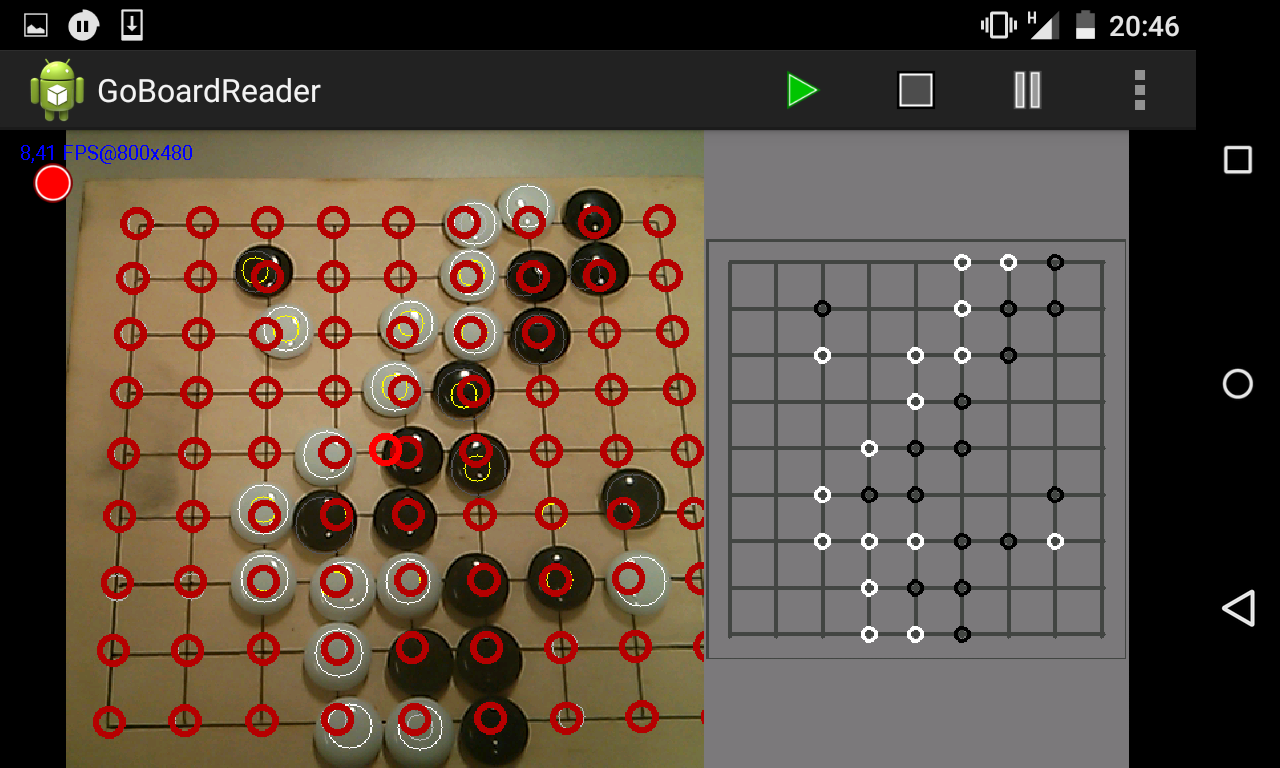
\includegraphics[width=0.7\textwidth]{images/android_ui.png}
		\caption{The app showing some debugging information and the detection result in a split screen while recording a game}
		\label{fig:android_ui}
	\end{figure}

	\subsection{Using the detection result}
	\label{android-detector-usingResults}
	Interestingly the computed intersections of two consecutive frames somewhat differ. On the one hand this very convenient: It helps dealing with specular highlights as the classification windows are constantly being shifted slightly. On the other hand sometimes the detection result will deteriorate completely. Even though the detector does some sanity checks, displaying and saving the detection results directly would result in pieces ``flickering'' between being detected and not. To counteract this we count the number of times an intersection was classified as white or black in the last ten frames. If this counter reaches 5 or higher we assume a correct result and display it. If the game is being recorded we also save two consecutive piece configurations in a list if they differ in at least one location.

	When the game ends we chose to simply save this list of char arrays as strings seperated by newlines as output format. This simple format allows easy transcoding and is even human readable.

	\section{User interaction design}
	\label{android-ui}
	The detection result still has to be displayed to the user. While often computer vision applications draw directly onto the analyzed image we decided to show the detected information separately and only debugging output on the image. This way we balance showcasing a possible way how an app might be responding to the user and also give an insight of whether and how the detector works.

	Android offers methods to draw custom views via \texttt{Canvas} and \texttt{Paint} objects similarly to OpenCV. However we wanted to give a comparable experience when using the detector on a desktop computer and via the app. Thus we decided to draw the result by cropping the input image and draw the result next to it using OpenCV when in detection mode.

	We furthermore implemented a replay mode in which previously recorded games can be stepped through move by move. This allows direct control over the detection result and is a simple way to recapitulate a game.
